\scanpage{93}
\mspage{\unsure{R|B}}
les \deleted{\unsure{en}} ensembles finis à opér. $\Pi_P^\tau$ — i.e. munis d'endomorphismes \deleted{$\tau_a\ (a\in A)$} involutifs $\tau_a$, indexés par les \uline{côtés} de $P$ — s'interprètent en termes de telles cartes, mais en supposant que les $\tau_a$ opèrent sans points fixes. \deleted{Pour \unsure{cela}}

\margin{Une pondération du type $P$}

Si on associe à la carte $X$ $P$-pondérée l'ensemble \inserted{$R(X)$} de ses \uline{faces}, on trouve en effet un ensemble avec des opérations $\tau_a$, \inserted{où $\tau_a$} correspondant \deleted{\unsure{une}} \inserted{à la} symétrie par r. \deleted{aux} à l'arête de type $a$ d'une face. Ici, la pondération (disons, numérotation circulaire) des \deleted{\uline{faces}} \inserted{\uline{arêtes} d'une \uline{face}} apparaît plus commode que celle des sommets. Le foncteur

\figure{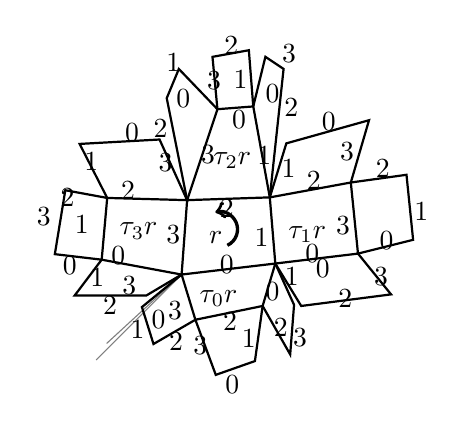
\begin{tikzpicture}[scale=.7]
\coordinate (A) at (0,0); \coordinate (B) at (1.5,.05);
\coordinate (C) at (1.6,-1.15); \coordinate (D) at (-.1,-1.35);
\draw[gray,thin] (D)--(-1.65,-2.9);
\draw[gray,thin] (D)--(-1.46,-2.6);
\draw[thick] (A)--(B)--(C)--(D)--cycle;
\draw[thick] (A)--(.55,1.65)--(1.2,1.7)--(B);
\draw[thick] (.55,1.65)--(.46,2.6)--(1.12,2.72)--(1.2,1.7);
\draw[thick] (A)--(-.37,1.85)--(-.15,2.38)--(.55,1.65);
\draw[thick] (B)--(1.75,2.38)--(1.42,2.6)--(1.2,1.7);
\draw[thick] (A)--(-1.45,.04)--(-1.95,1.02)--(-.5,1.1)--cycle;
\draw[thick] (-1.45,.04)--(-1.55,-1.08)--(D);
\draw[thick] (-1.45,.04)--(-2.21,.18)--(-2.4,-.98)--(-1.55,-1.08);
\draw[thick] (-1.55,-1.08)--(-2.04,-1.73)--(-.74,-1.73)--(D);
\draw[thick] (D)--(.15,-2.17)--(1.37,-1.92)--(C);
\draw[thick] (.15,-2.17)--(.52,-3.17)--(1.23,-2.92)--(1.37,-1.92);
\draw[thick] (D)--(-.82,-1.94)--(-.61,-2.61)--(.15,-2.17);
\draw[thick] (C)--(1.94,-1.9)--(1.87,-2.8)--(1.37,-1.92);
\draw[thick] (B)--(2.97,.32)--(3.1,-.97)--(C);
\draw[thick] (B)--(1.8,1.03)--(3.3,1.45)--(2.97,.32);
\draw[thick] (2.97,.32)--(3.98,.46)--(4.1,-.72)--(3.1,-.97);
\draw[thick] (C)--(2.07,-1.92)--(3.7,-1.71)--(3.1,-.97);
\node at (.52,-.68) {$r$};
\draw[very thick,->] (.73,-.82) arc[start angle=-65,end angle=105,radius=.32];
\node at (.82,.72) {$\tau_2r$};
\node at (-.88,-.56) {$\tau_3r$};
\node at (2.18,-.62) {$\tau_1r$};
\node at (.57,-1.78) {$\tau_0r$};
\foreach \x/\y/\z in {
.72/-.15/2,1.35/-.68/1,.72/-1.17/0,-.25/-.63/3,
.94/1.47/0,.38/.82/3,1.4/.81/1,
.49/2.17/3,.97/2.18/1,.8/2.8/2,
-.07/1.85/0,-.48/1.3/2,-.25/2.5/1,
1.55/1.94/0,1.89/1.68/2,1.85/2.66/3,
-1.07/.17/2,-1/1.23/0,-1.74/.7/1,-.39/.68/3,
-1.25/-1/0,-1.91/-.45/1,-2.17/.05/2,-2.6/-.3/3,-2.13/-1.18/0,
-1.63/-1.41/1,-1.05/-1.55/3,-1.4/-1.91/2,
-.52/-2.16/0,-.22/-2/3,-.9/-2.35/1,-.2/-2.57/2,
.78/-2.2/2,1.12/-2.52/1,.24/-2.63/3,.82/-3.35/0,
1.55/-1.65/0,1.7/-2.32/2,2.05/-2.5/3,1.9/-1.38/1,
2.27/-.97/0,2.83/-.47/3,
1.84/.58/1,2.3/.35/2,2.9/.89/3,2.57/1.43/0,
3.55/.57/2,4.25/-.2/1,3.62/-.73/0,
2.46/-1.24/0,2.87/-1.79/2,3.52/-1.38/3}
{\node at (\x,\y) {$\z$};}
\end{tikzpicture}}

\diagram{\begin{tikzcd}[ampersand replacement=\&,column sep=large]
X\arrow[r,mapsto]\&R(X)\\
\begin{gathered}\text{cartes $P$-pondérées}\\\text{finies}\\(\text{cat. isotopique})\end{gathered}
\arrow[r,"\approx"]\&
\begin{gathered}\Pi_P^\tau\text{-ensembles finis}\\\text{spéciaux}\\
(\text{i.e. où les }\tau_i\\\text{opèrent ss pt fixe})\end{gathered}
\end{tikzcd}}
(\unsure{100|101})

est une équivalence des catégories. \deleted{L'équivalence} \inserted{Elle induit une équivalence}
\deleted{qui \unsure{à un} \unsure{$N$} \unsure{vient} \unsure{on associe à} $N$}
\deleted{$\Pi_P^\tau$-\unsure{ensembles}}

\diagram{\begin{tikzcd}[ampersand replacement=\&,column sep=large]
\begin{gathered}\text{cartes $P$-pondérées }\deleted{\text{étales}}\\\text{finies \uline{orientées}}\end{gathered}
\arrow[r,"\approx"]\&
\Pi_P\text{-ens. finis}\\
\&X\arrow[r,mapsto]\&R^+(X)
\end{tikzcd}}
(102)

en associant à chaque telle carte l'ens $R^+(X)$ de ses \deleted{repères} faces ``directes'', i.e. \deleted{que} dont l'orientation induite par $X$ est celle définie par $\omega\in\underline\omega$, définissant un ordre circulaire sur l'ens des sommets (ou des arêtes)

\margin{92}
